\documentclass[pdftex,twocolumn,epjc3]{svjour3}

\usepackage{fontenc}
\usepackage{calc}
\usepackage{graphicx}
\usepackage{booktabs}
\usepackage{textcomp}
\usepackage{xspace}
\usepackage{relsize}
\usepackage{amssymb}
\usepackage{amsmath}
\usepackage{listings}
\usepackage{microtype}
\usepackage{multirow}
\usepackage{tabularx}
\usepackage{array}
\usepackage[utf8]{inputenc}
\usepackage[numbers,sort&compress]{natbib}
\usepackage[labelfont=bf,font=small]{caption}
\usepackage[skip=-2pt]{subcaption}
\usepackage[colorlinks,citecolor=blue,urlcolor=blue,linkcolor=blue]{hyperref}
\usepackage[usenames,dvipsnames]{xcolor}
\usepackage[clockwise,figuresright]{rotating}

\newcolumntype{L}{>{\raggedright\let\newline\\\arraybackslash\hspace{0pt}}X}
\newcolumntype{R}{>{\raggedleft\let\newline\\\arraybackslash\hspace{0pt}}X}
\newcolumntype{C}{>{\centering\let\newline\\\arraybackslash\hspace{0pt}}X}

\setlength{\rotFPtop}{0pt plus 1fil}
\setcounter{tocdepth}{3}

\makeatletter
% \DeclareRobustCommand{\kbd}[1]{{\texttt{#1}}}
% \DeclareRobustCommand{\code}[1]{\kbd{#1}\xspace}
% \DeclareRobustCommand{\To}{\ensuremath{\Rightarrow}\xspace}
\g@addto@macro\bfseries{\boldmath}
\makeatother

\newcommand{\subparagraph}{} %< workaround for svjour not defining subparagraph
\usepackage{titlesec}
% \titleformat*{\section}{\Large\bfseries\sffamily}
% \titleformat*{\subsection}{\large\bfseries\sffamily}
% \titleformat*{\subsubsection}{\bfseries\sffamily}
\titleformat*{\paragraph}{\bfseries}
% \titleformat*{\subparagraph}{\slshape}
% \titlespacing*{\section}{0pt}{3ex plus .2ex minus .2ex}{1ex plus .2ex}
% \titlespacing*{\subsection}{0pt}{3ex plus .4ex minus .4ex}{0.8ex plus .2ex}
% \titlespacing*{\subsubsection}{0pt}{1.5ex plus .2ex minus .2ex}{0.5ex plus .2ex}
% \titlespacing*{\paragraph}{0pt}{1ex plus .1ex minus .1ex}{0.5ex plus .1ex minus .1ex}
% \titlespacing*{\subparagraph}{0pt}{0ex plus .1ex minus .1ex}{0.5ex plus .1ex minus .1ex}

\journalname{Eur. Phys. J. C}
\bibliographystyle{JHEP_pat}
\smartqed
\sloppy

\let\underscore\_
\renewcommand{\_}{\discretionary{\underscore}{}{\underscore}}

\makeatletter
\let\orgdescriptionlabel\descriptionlabel
\renewcommand*{\descriptionlabel}[1]{%
  \let\orglabel\label
  \let\label\@gobble
  \phantomsection
  \protected@edef\@currentlabel{#1}%
  %\protected@edef\@currentlabelname{#1}
  \let\label\orglabel
  \orgdescriptionlabel{#1}%
}
\makeatother

%Journal definitions
% Bibliography and bibfile
\def\lnp{Lec.\ Notes in Physics}
          % Lecture Notes in Physics
\def\cpc{Comp.\ Phys.\ Comm.}
          % Computer Physics Communications
\def\jpg{J. Phys. G}
          % Journal of Physics G Nuclear Physics
\def\ijmpa{Int.\ J.\ Mod.\ Phys.\ A}
          % International Journal of Modern Physics A
\def\epjc{Eur.\ Phys.\ J.\ C}
          % European Physical Journal C
\def\nima{Nuc.\ Inst.\ Methods A}
          % Nuclear Instruments and Methods A
\def\nimb{Nuc.\ Inst.\ Methods B}
          % Nuclear Instruments and Methods B
\def\njp{New J.\ Phys.}
          % New Journal of Physics
\def\rmp{Rev.\ Mod.\ Phys.}
          % Reviews of Modern Physics
\def\app{Astropart.\ Phys.}
          % Astroparticle Physics
\def\aj{AJ}%
          % Astronomical Journal
\def\actaa{Acta Astron.}%
          % Acta Astronomica
\def\araa{ARA\&A}%
          % Annual Review of Astron and Astrophys
\def\arnps{Ann.~Rev.~Nucl.~\& Part.~Sci.}%
          % Annual Review of Astron and Astrophys
\def\apj{ApJ}%
          % Astrophysical Journal
\def\apjl{ApJ}%
          % Astrophysical Journal, Letters
\def\apjs{ApJS}%
          % Astrophysical Journal, Supplement
\def\ao{Appl.\ Opt.}%
          % Applied Optics
\def\apss{Ap\&SS}%
          % Astrophysics and Space Science
\def\aap{A\&A}%
          % Astronomy and Astrophysics
\def\aapr{A\&A~Rev.}%
          % Astronomy and Astrophysics Reviews
\def\aaps{A\&AS}%
          % Astronomy and Astrophysics, Supplement
\def\azh{AZh}%
          % Astronomicheskii Zhurnal
\def\pos{PoS}%
          % Proceedings of Science
\def\baas{BAAS}%
          % Bulletin of the AAS
\def\bac{Bull.\ Astr.\ Inst.\ Czechosl.}%
          % Bulletin of the Astronomical Institutes of Czechoslovakia 
\def\caa{Chinese Astron.\ Astrophys.}%
          % Chinese Astronomy and Astrophysics
\def\cjaa{Chinese J.\ Astron.\ Astrophys.}%
          % Chinese Journal of Astronomy and Astrophysics
\def\icarus{Icarus}%
          % Icarus
\def\jhep{JHEP}%
          % Journal of High Energy Physics
\def\jcap{JCAP}%
          % Journal of Cosmology and Astroparticle Physics
\def\jpsj{J.\ Phys.\ Soc.\ Japan}%
          % Journal of the Physical Society of Japan
\def\jrasc{JRASC}%
          % Journal of the RAS of Canada
\def\canjphys{Can.~J.~Phys.}
          %Canadian Journal of Physics
\def\apphys{Astropart.~Phys.}
          %Astroparticle Physics
\def\mnras{MNRAS}%
          % Monthly Notices of the RAS
\def\memras{MmRAS}%
          % Memoirs of the RAS
\def\na{New A}%
          % New Astronomy
\def\nar{New A Rev.}%
          % New Astronomy Review
\def\pasa{PASA}%
          % Publications of the Astron. Soc. of Australia
\def\pra{Phys.\ Rev.\ A}%
          % Physical Review A: General Physics
\def\prb{Phys.\ Rev.\ B}%
          % Physical Review B: Solid State
\def\prc{Phys.\ Rev.\ C}%
          % Physical Review C
\def\prd{Phys.\ Rev.\ D}%
          % Physical Review D
\def\pre{Phys.\ Rev.\ E}%
          % Physical Review E
\def\prl{Phys.\ Rev.\ Lett.}%
          % Physical Review Letters
\def\pasp{PASP}%
          % Publications of the ASP
\def\pasj{PASJ}%
          % Publications of the ASJ
\def\qjras{QJRAS}%
          % Quarterly Journal of the RAS
\def\rmxaa{Rev. Mexicana Astron. Astrofis.}%
          % Revista Mexicana de Astronomia y Astrofisica
\def\skytel{S\&T}%
          % Sky and Telescope
\def\solphys{Sol.\ Phys.}%
          % Solar Physics
\def\sovast{Soviet~Ast.}%
          % Soviet Astronomy
\def\ssr{Space~Sci.\ Rev.}%
          % Space Science Reviews
\def\zap{ZAp}%
          % Zeitschrift fuer Astrophysik
\def\nat{Nature}%
          % Nature
\def\science{Science}%
\def\sci{\science}%
          % Science
\def\iaucirc{IAU~Circ.}%
          % IAU Cirulars
\def\aplett{Astrophys.\ Lett.}%
          % Astrophysics Letters
\def\apspr{Astrophys.\ Space~Phys.\ Res.}%
          % Astrophysics Space Physics Research
\def\bain{Bull.\ Astron.\ Inst.\ Netherlands}%
          % Bulletin Astronomical Institute of the Netherlands
\def\fcp{Fund.\ Cosmic~Phys.}%
          % Fundamental Cosmic Physics
\def\gca{Geochim.\ Cosmochim.\ Acta}%
          % Geochimica Cosmochimica Acta
\def\grl{Geophys.\ Res.\ Lett.}%
          % Geophysics Research Letters
\def\jcp{J.\ Chem.\ Phys.}%
          % Journal of Chemical Physics
\def\jgr{J.\ Geophys.\ Res.}%
          % Journal of Geophysics Research
\def\jqsrt{J.\ Quant.\ Spec.\ Radiat.\ Transf.}%
          % Journal of Quantitiative Spectroscopy and Radiative Trasfer
\def\memsai{Mem.\ Soc.\ Astron.\ Italiana}%
          % Mem. Societa Astronomica Italiana
\def\nphysa{Nucl.\ Phys.\ A}%
          % Nuclear Physics A
\def\nphysb{Nucl.\ Phys.\ B}%
          % Nuclear Physics B
\def\physrep{Phys.\ Rep.}%
          % Physics Reports
\def\physscr{Phys.\ Scr}%
          % Physica Scripta
\def\planss{Planet.\ Space~Sci.}%
          % Planetary Space Science
\def\procspie{Proc.\ SPIE}%
          % Proceedings of the SPIE
\def\repprogphys{Rep.\ Prog.\ Phys.}%
          % Reports of Progress in Physics
\def\jpcrd{J. Phys. Chem. Ref. Data}% 
        %Journal of Physical and Chemical Reference Data 
\def\jphysb{J. Phys. B}% 
	%Journal of Physics B Atomic Molecular Physics
\def\jphysd{J. Phys. D}% 
	%Journal of Physics D
\def\jphysconfseries{J. Phys. Conf. Series}% 
	%Journal of Physics: Conference Series
\def\physrev{\pr}
\def\pr{Phys. Rev.}% 
	%Physical Review
\def\josa{J. Opt. Soc. Amer. (1917-1983)}% 
	%Journal of the Optical Society of America (1917-1983) 
\def\josab{J. Opt. Soc. Amer. B}% 
	%Journal of the Optical Society of America B Optical Physics
\def\pla{Phys. Lett. A}% 
	%Physics Letters A
\def\plb{Phys. Lett. B}% 
	%Physics Letters B
\def\os{Opt. Spectrosc. (Russ.)}% 
	%Optics and Spectroscopy (Russ. / USSR)
\def\jas{J. Appl. Spectrosc.}% 
	%Journal of Applied Spectroscopy (Russ. / USSR)
\def\annp{Ann. Phys.}% 
	%Annalen der Physik
\def\sa{Spectrochim. Acta}% 
	%Spectrochimica Acta
\def\prsoca{Proc. R. Soc. London Ser. A}% 
	%Proceedings of the Royal Society of London, Series A
\def\zphysa{Z. Phys. A}% 
	%Zeitschrift fur Physik A
\def\zphysb{Z. Phys. B}% 
	%Zeitschrift fur Physik B
\def\zphysc{Z. Phys. C}% 
	%Zeitschrift fur Physik C
\def\zphysd{Z. Phys. D}% 
	%Zeitschrift fur Physik D
\def\zphyse{Z. Phys. E}% 
	%Zeitschrift fur Physik E
\def\zphys{Z. Phys.}% 
	%Zeitschrift fur Physik
\def\adndt{Atom. Data Nuc. Data Tables}% 
	%Atomic Data and Nuclear Data Tables
\def\jmolspec{J. Mol. Spectrosc.}% 
	%Journal of Molecular Spectroscopy
\def\aphysb{Appl. Phys. B}% 
	%Applied Physics B: Lasers and Optics
\def\nim{Nuc. Inst. Meth.}% 
	%Nuclear Instruments and Methods
\def\jphysique{J. Phys. (Paris)}% 
	%Journal de Physique
\def\epjp{Eur.~Phys.~J.~Plus}%
        %European Physical Journal Plus
\def\epjc{Eur.~Phys.~J.~C}%
        %European Physical Journal C
\def\epl{Europhys.~Lett}%
        %Europhysics Letters
\def\njp{New J.~Phys.}
        %New Journal of Physics
\let\astap=\aap
\let\apjlett=\apjl
\let\apjsupp=\apjs
\let\applopt=\ao
%


\newcommand\cpp[1]{\lstinline{#1}}
\newcommand\yaml[1]{\lstset{style=yaml}\lstinline{#1}\lstset{style=cpp}}
\newcommand\yamlvalue[1]{{\YAMLvaluestyle\ttfamily#1}}
\newcommand\term[1]{\lstset{style=terminal}\lstinline{#1}\lstset{style=cpp}}
\newcommand\fortran[1]{\lstset{style=fortran}\lstinline{#1}\lstset{style=cpp}}
\newcommand\py[1]{\lstset{style=python}\lstinline{#1}\lstset{style=cpp}}

% Ben: Placeholder command for referring to glossary items in core paper from other paper
\newcommand\corejargon[1]{\textbf{#1}}

\lstnewenvironment{lstlistingyaml}{\lstset{style=yaml}}{\lstset{style=cpp}}
\lstnewenvironment{lstlistingterm}{\lstset{style=terminal}}{\lstset{style=cpp}}
\lstnewenvironment{lstlistingfortran}{\lstset{style=fortran}}{\lstset{style=cpp}}
\lstnewenvironment{lstcpp}{\lstset{style=cpp}}{\lstset{style=cpp}}
\lstnewenvironment{lstcppalt}{\lstset{style=cppalt}}{\lstset{style=cpp}}
\lstnewenvironment{lstcppnum}{\lstset{style=cppnum}}{\lstset{style=cpp}}
\lstnewenvironment{lstyaml}{\lstset{style=yaml}}{\lstset{style=cpp}}
\lstnewenvironment{lstterm}{\lstset{style=terminal}}{\lstset{style=cpp}}
\lstnewenvironment{lsttermalt}{\lstset{style=terminalalt}}{\lstset{style=cpp}}
\lstnewenvironment{lstfortran}{\lstset{style=fortran}}{\lstset{style=cpp}}
\lstnewenvironment{lstpy}{\lstset{style=python}}{\lstset{style=cpp}}

%C++ syntax highlighting, direct from http://marcusmo.co.uk/blog/latex-syntax-highlighting/
% Solarized colour scheme for listings
\definecolor{solarized@base03}{HTML}{002B36}
\definecolor{solarized@base02}{HTML}{073642}
\definecolor{solarized@base01}{HTML}{586e75}
\definecolor{solarized@base00}{HTML}{657b83}
\definecolor{solarized@base0}{HTML}{839496}
\definecolor{solarized@base1}{HTML}{93a1a1}
\definecolor{solarized@base2}{HTML}{EEE8D5}
\definecolor{solarized@base3}{HTML}{FDF6E3}
\definecolor{solarized@yellow}{HTML}{B58900}
\definecolor{solarized@orange}{HTML}{CB4B16}
\definecolor{solarized@red}{HTML}{DC322F}
\definecolor{solarized@magenta}{HTML}{D33682}
\definecolor{solarized@violet}{HTML}{6C71C4}
\definecolor{solarized@blue}{HTML}{268BD2}
\definecolor{solarized@cyan}{HTML}{2AA198}
\definecolor{solarized@green}{HTML}{859900}
\definecolor{darkred}{HTML}{550003}
\newcommand\YAMLcolonstyle{\footnotesize\color{solarized@red}\mdseries}
\newcommand\YAMLstringstyle{\footnotesize\color{solarized@green}\mdseries}
\newcommand\YAMLkeystyle{\footnotesize\color{solarized@blue}\ttfamily}
\newcommand\YAMLvaluestyle{\footnotesize\color{blue}\mdseries}
\newcommand\ProcessThreeDashes{\llap{\color{cyan}\mdseries-{-}-}}
% Define C++ syntax highlighting colour scheme
\newcommand\CPPplainstyle{\footnotesize\ttfamily}
\newcommand\CPPkeywordstyle{\color{solarized@orange}\footnotesize\ttfamily}
\newcommand\CPPidentifierstyle{\color{solarized@blue}\footnotesize\ttfamily}
\lstdefinestyle{cpp}
{
  language=C++,
  basicstyle=\footnotesize\ttfamily,
  basewidth={0.53em,0.44em}, %Ben: experimenting a bit with the fixed-width width (first argument); feels a bit more readable to me with the slightly smaller width (was 0.6em by default)
  numbers=none,
  tabsize=2,
  breaklines=true,
  escapeinside={@}{@},
  showstringspaces=false,
  numberstyle=\tiny\color{solarized@base01},
  keywordstyle=\color{solarized@orange},
  stringstyle=\color{solarized@red}\ttfamily,
  identifierstyle=\color{solarized@blue},
  commentstyle=\color{solarized@violet},
  morecomment=[l]{\#pragma},
  emphstyle=\color{solarized@green},
  frame=single,
  rulecolor=\color{solarized@base2},
  rulesepcolor=\color{solarized@base2},
  otherkeywords={\#define,\#undef,\#include},
  literate =
}
% C++ style with different escape character (so I can use @'s in strings)
\lstdefinestyle{cppalt}
{
  language=C++,
  basicstyle=\footnotesize\ttfamily,
  basewidth={0.53em,0.44em}, %Ben: experimenting a bit with the fixed-width width (first argument); feels a bit more readable to me with the slightly smaller width (was 0.6em by default)
  numbers=none,
  tabsize=2,
  breaklines=true,
  escapeinside={*@}{@*},
  showstringspaces=false,
  numberstyle=\tiny\color{solarized@base01},
  keywordstyle=\color{solarized@orange},
  stringstyle=\color{solarized@red}\ttfamily,
  identifierstyle=\color{solarized@blue},
  commentstyle=\color{solarized@violet},
  emphstyle=\color{solarized@green},
  frame=single,
  rulecolor=\color{solarized@base2},
  rulesepcolor=\color{solarized@base2},
  otherkeywords={define,undef,include,\#},
  literate =
}
% C++ style with line numbers (try to keep everything else matching the 'cpp' style)
\lstdefinestyle{cppnum}
{
  language=C++,
  basicstyle=\footnotesize\ttfamily,
  basewidth={0.53em,0.44em}, %Ben: experimenting a bit with the fixed-width width (first argument); feels a bit more readable to me with the slightly smaller width (was 0.6em by default)
  numbers=left,
  tabsize=2,
  breaklines=true,
  escapeinside={@}{@},
  showstringspaces=false,
  numberstyle=\tiny\color{solarized@base01},
  keywordstyle=\color{solarized@orange},
  stringstyle=\color{solarized@red}\ttfamily,
  identifierstyle=\color{solarized@blue},
  commentstyle=\color{solarized@violet},
  emphstyle=\color{solarized@green},
  frame=single,
  rulecolor=\color{solarized@base2},
  rulesepcolor=\color{solarized@base2},
  otherkeywords={define,undef,include,\#},
  literate =
}
% Define python syntax highlighting colour scheme
\lstdefinestyle{python}
{
  language=Python,
  basicstyle=\footnotesize\ttfamily,
  basewidth={0.53em,0.44em},
  numbers=none,
  tabsize=2,
  breaklines=true,
  escapeinside={@}{@},
  showstringspaces=false,
  numberstyle=\tiny\color{solarized@base01},
  keywordstyle=\color{blue},
  stringstyle=\color{orange}\ttfamily,
  identifierstyle=\color{darkred},
  commentstyle=\color{purple},
  emphstyle=\color{green},
  frame=single,
  rulecolor=\color{solarized@base2},
  rulesepcolor=\color{solarized@base2},
  literate = {\ as\ }{{\color{blue}\ as\ }}3 
}
% Define fortran syntax highlighting colour scheme
\lstdefinestyle{fortran}
{
  language=Fortran,
  basicstyle=\footnotesize\ttfamily,
  basewidth={0.53em,0.44em},
  numbers=none,
  tabsize=2,
  breaklines=true,
  escapeinside={@}{@},
  showstringspaces=false,
  numberstyle=\tiny\color{solarized@base01},
  keywordstyle=\color{blue},
  stringstyle=\color{orange}\ttfamily,
  identifierstyle=\color{black},
  commentstyle=\color{purple},
  emphstyle=\color{green},
  frame=single,
  rulecolor=\color{solarized@base2},
  rulesepcolor=\color{solarized@base2},
}
% Define shell syntax highlighting colour scheme
% Ben: I cannot get the damn comment highlighting to work for the 'bash' language. No idea what the problem is, the internet seems to think that it should just work.
\lstdefinestyle{terminal}
{
  language=bash,
  basicstyle=\footnotesize\ttfamily,
  numbers=none,
  tabsize=2,
  breaklines=true,
  escapeinside={@}{@},
  frame=single,
  showstringspaces=false,
  numberstyle=\tiny\color{solarized@base01},
  keywordstyle=\color{solarized@orange},
  stringstyle=\color{solarized@red}\ttfamily,
  identifierstyle=\color{black},
  commentstyle=\color{solarized@violet},
  emphstyle=\color{solarized@green},
  frame=single,
  rulecolor=\color{solarized@base2},
  rulesepcolor=\color{solarized@base2},
  morekeywords={gambit, cmake, make, mkdir},
  deletekeywords={test},
  literate = {\ gambit}{{\ }{\color{black}}gambit}7
             {/gambit}{{/}{\color{black}}gambit}6
             {/include}{{/}{\color{black}}include}8
             {cmake/}{{\color{black}}cmake/}6
             {.cmake}{{.}{\color{black}}cmake}6
}
% Terminal style with alternate escape character
\lstdefinestyle{terminalalt}
{
  language=bash,
  basicstyle=\footnotesize\ttfamily,
  numbers=none,
  tabsize=2,
  breaklines=true,
  escapeinside={*@}{@*},
  frame=single,
  showstringspaces=false,
  numberstyle=\tiny\color{solarized@base01},
  keywordstyle=\color{solarized@orange},
  stringstyle=\color{solarized@red}\ttfamily,
  identifierstyle=\color{black},
  commentstyle=\color{solarized@violet},
  emphstyle=\color{solarized@green},
  frame=single,
  rulecolor=\color{solarized@base2},
  rulesepcolor=\color{solarized@base2},
  morekeywords={gambit, cmake, make, mkdir},
  deletekeywords={test},
  literate = {\ gambit}{{\ }{\color{black}}gambit}7
             {/gambit}{{/}{\color{black}}gambit}6
             {/include}{{/}{\color{black}}include}8
             {cmake/}{{\color{black}}cmake/}6
             {.cmake}{{.}{\color{black}}cmake}6
}
\newcommand{\negphantom}[1]{\settowidth{\dimen0}{#1}\hspace*{-\dimen0}}
% Define yaml syntax highlighting colour scheme
\lstdefinestyle{yaml}
{
  escapeinside={@}{@},
  keywords={true,false,null},
  otherkeywords={},
  keywordstyle=\color{solarized@base0}\bfseries,
  basicstyle=\footnotesize\color{black}\ttfamily,
  identifierstyle=\YAMLkeystyle,
  sensitive=false,
  commentstyle=\color{solarized@orange}\ttfamily,
  morecomment=[l]{\#},
  morecomment=[s]{/*}{*/},
  stringstyle=\YAMLstringstyle\ttfamily,
  moredelim=**[s][\YAMLkeystyle]{,}{:},   % switch to value style at : but back to key style at,
  moredelim=**[l][\YAMLvaluestyle]{:},    % switch to value style at :
  morestring=[b]',
  morestring=[b]",
  literate =    {---}{{\ProcessThreeDashes}}3
                {>}{{\textcolor{solarized@red}\textgreater}}1
                {|}{{\textcolor{solarized@red}\textbar}}1
                {\ -\ }{{\mdseries\color{black}\ -\ \negmedspace}}3
                {\}}{{{\color{black} \}}}}1
                {\{}{{{\color{black} \{}}}1
                {[}{{{\color{black} [}}}1
                {]}{{{\color{black} ]}}}1,
  breakindent=0pt,
  breakatwhitespace,
  columns=fullflexible
}
% Start with C++ style on
\lstset{style=cpp}

% Glossary commands
\newcommand{\cross}[1]{\ref{#1}}
\newcommand{\doublecross}[2]{\hyperref[#2]{\textbf{#1}}}
\newcommand{\doublecrosssf}[2]{\hyperref[#2]{\textbf{\textsf{#1}}}}
\newcommand{\gitem}[1]{\item[\textbf{#1}\label{#1}]}
\newcommand{\gsfitem}[1]{\item[\textbf{\textsf{#1}}\label{#1}]}

% Code commands
\newcommand{\bcode}{\begin{lstlisting}}
\newcommand{\ecode}{\end{lstlisting}}
\newcommand{\metavar}[1]{\textit{\color{black!70}\footnotesize\textrm{#1}}}

% For sign(mu), etc.
\DeclareMathOperator{\sign}{sign}

% Physics units
\newcommand{\eV}{\ensuremath{\text{e}\mspace{-0.8mu}\text{V}}\xspace}
\newcommand{\MeV}{\text{M\eV}\xspace}
\newcommand{\GeV}{\text{G\eV}\xspace}
\newcommand{\TeV}{\text{T\eV}\xspace}
\newcommand{\pb}{\text{pb}\xspace}
\newcommand{\fb}{\text{fb}\xspace}
\newcommand{\invpb}{\ensuremath{\pb^{-1}}\xspace}
\newcommand{\invfb}{\ensuremath{\fb^{-1}}\xspace}

% Physical quantities
\newcommand{\pt}{\ensuremath{p_\mathrm{T}}\xspace}
\newcommand{\et}{\ensuremath{E_\mathrm{T}}\xspace}
\newcommand{\etmiss}{\ensuremath{E_\mathrm{T}^\mathrm{\mspace{1.5mu}miss}}\xspace}
\newcommand{\hT}{\ensuremath{H_\mathrm{T}}\xspace}
\newcommand{\dphi}{\ensuremath{\Delta\phi}\xspace}
\newcommand{\lhs}{\lambda_{h\sss S}}
\newcommand{\ls}{\lambda_{\sss S}}
\newcommand{\DR}{$\overline{DR}$\xspace}
\newcommand{\MSbar}{$\overline{MS}$\xspace}

% Textual shortcuts
\newcommand{\ie}{\textit{i.e.}\ }
\newcommand{\eg}{\textit{e.g.}\ }
\newcommand{\atlas}{ATLAS\xspace}
\newcommand{\cms}{CMS\xspace}
\newcommand{\gambit}{\textsf{GAMBIT}\xspace}
\newcommand{\darkbit}{\textsf{DarkBit}\xspace}
\newcommand{\colliderbit}{\textsf{ColliderBit}\xspace}
\newcommand{\flavbit}{\textsf{FlavBit}\xspace}
\newcommand{\specbit}{\textsf{SpecBit}\xspace}
\newcommand{\decaybit}{\textsf{DecayBit}\xspace}
\newcommand{\precisionbit}{\textsf{PrecisionBit}\xspace}
\newcommand{\scannerbit}{\textsf{ScannerBit}\xspace}
\newcommand{\examplebita}{\textsf{ExampleBit\_A}\xspace}
\newcommand{\examplebitb}{\textsf{ExampleBit\_B}\xspace}
\newcommand{\BOSS}{\textsf{BOSS}\xspace}
\newcommand{\GB}{\gambit}
\newcommand{\DB}{\darkbit}
\newcommand{\omp}{\textsf{OpenMP}\xspace}
\newcommand{\openmpi}{\textsf{OpenMPI}\xspace}
\newcommand{\mpi}{\textsf{MPI}\xspace}
\newcommand{\posix}{\textsf{POSIX}\xspace}
\newcommand{\buckfast}{\textsf{BuckFast}\xspace}
\newcommand{\delphes}{\textsf{Delphes}\xspace}
\newcommand{\pythia}{\textsf{Pythia}\xspace}
\newcommand{\pythiaeight}{\textsf{Pythia 8}\xspace}
\newcommand{\PythiaEM}{\textsf{PythiaEM}\xspace}
\newcommand{\prospino}{\textsf{Prospino}\xspace}
\newcommand{\nllfast}{\textsf{NLL-fast}\xspace}
\newcommand{\madgraph}{\textsf{MadGraph}\xspace}
\newcommand{\fastjet}{\textsf{FastJet}\xspace}
\newcommand{\smodels}{\textsf{SmodelS}\xspace}
\newcommand{\fastlim}{\textsf{Fastlim}\xspace}
\newcommand{\checkmate}{\textsf{CheckMATE}\xspace}
\newcommand{\higgsbounds}{\textsf{HiggsBounds}\xspace}
\newcommand{\susypope}{\textsf{SUSYPope}\xspace}
\newcommand{\higgssignals}{\textsf{HiggsSignals}\xspace}
\newcommand{\ds}{\textsf{DarkSUSY}\xspace}
\newcommand{\pppc}{\textsf{PPPC4DMID}\xspace}
\newcommand{\micromegas}{\textsf{micrOMEGAs}\xspace}
\newcommand{\rivet}{\textsf{Rivet}\xspace}
\newcommand{\feynrules}{\textsf{Feynrules}\xspace}
\newcommand{\feynhiggs}{\textsf{FeynHiggs}\xspace}
\newcommand\SARAH{\textsf{SARAH}\xspace}
\newcommand\SPheno{\textsf{SPheno}\xspace}
\newcommand\superiso{\textsf{SuperIso}\xspace}
\newcommand\FlexibleSUSY{\textsf{FlexibleSUSY}\xspace}
\newcommand\SOFTSUSY{\textsf{SOFTSUSY}\xspace}
\newcommand\SUSPECT{\textsf{SUSPECT}\xspace}
\newcommand\NMSSMCalc{\textsf{NMSSMCALC}\xspace}
\newcommand\NMSSMTools{\textsf{NMSSMTools}\xspace}
\newcommand\NMSPEC{\textsf{NMSPEC}\xspace}
\newcommand\NMHDECAY{\textsf{NMHDECAY}\xspace}
\newcommand\HDECAY{\textsf{HDECAY}\xspace}
\newcommand\SDECAY{\textsf{SDECAY}\xspace}
\newcommand\SUSYHIT{\textsf{SUSYHIT}\xspace}
\newcommand\SFOLD{\textsf{SFOLD}\xspace}
\newcommand\HFOLD{\textsf{HFOLD}\xspace}
\newcommand\FeynHiggs{\textsf{FeynHiggs}\xspace}
\newcommand\Mathematica{\textsf{Mathematica}\xspace}
\newcommand\lilith{\textsf{Lilith}\xspace}
\newcommand\nulike{\textsf{nulike}\xspace}
\newcommand\gamLike{\textsf{gamLike}\xspace}
\newcommand\pippi{\textsf{pippi}\xspace}
\newcommand\MultiNest{\textsf{MultiNest}\xspace}
\newcommand\gamlike{\textsf{GamLike}\xspace}
\newcommand\ddcalc{\textsf{DDCalc}\xspace}
\newcommand\xx{\raisebox{0.2ex}{\smaller ++}\xspace}
\newcommand\Cpp{\textsf{C\xx}\xspace}
\newcommand\Cppeleven{\textsf{C\raisebox{0.2ex}{\smaller ++}11}\xspace}
\newcommand\plainC{\textsf{C}\xspace}
\newcommand\Python{\textsf{Python}\xspace}
\newcommand\python{\Python}
\newcommand\Fortran{\textsf{Fortran}\xspace}

\newcommand{\beq}{\equation}
\newcommand{\eeq}{\endequation}
\newcommand{\sss}{\scriptscriptstyle}
\newcommand{\ms}{m_{\sss S}}
\newcommand{\mail}[1]{\href{mailto:#1}{#1}}

% Author comments
\newcommand{\TODO}[1]{\textbf{\textcolor{red}{#1}}}
\newcommand{\tb}[1]{{\color{green}\textbf{[TB: #1]}}}
\newcommand{\ps}[1]{\Pat{: #1}}
\newcommand{\cw}[1]{{\color{red}Christoph: #1}}
\newcommand{\gm}[1]{{\color{violet}Greg: #1}}
\newcommand{\Ben}[1]{{\bf\color{magenta}Ben #1}}
\newcommand{\Csaba}[1]{{\bf\color{orange}Csaba #1}}
\newcommand{\Chris}[1]{{\bf\color{olive}Chris #1}}
\newcommand{\Pat}[1]{{\bf\color{blue}Pat #1}}
\newcommand{\Peter}[1]{{\bf\color{purple}Peter #1}}
\newcommand{\Anders}[1]{{\bf\color{brown}Anders #1}}
\newcommand{\James}[1]{{\bf\color{teal}James #1}}
\newcommand{\Abram}[1]{{\bf\color{black!20!gray!60!magenta}Abram: #1}}

% Custom \chapter-like command  (svjour3 document class does not define \part or \chapter)
\newcommand{\segment}[1]{
 {\clearpage\noindent\phantomsection\huge\it#1\par}
 {\addcontentsline{toc}{section}{\it#1}}
}


\begin{document}

\def\A{\mathcal{A}}
\def\B{\mathcal{B}}
\def\C{\mathcal{C}}

\newcommand{\mb}{\textsf{Mass Builder} }
\newcommand{\mbs}{\textsf{Mass Builder}}
\newcommand{\tsil}{\textsf{TSIL} }
\newcommand{\tsils}{\textsf{TSIL}}
\newcommand{\tarcer}{\textsf{TARCER} }
\newcommand{\tarcers}{\textsf{TARCER}}
\newcommand{\sarah}{\textsf{SARAH} }
\newcommand{\sarahs}{\textsf{SARAH}}
\newcommand{\feynarts}{\textsf{FeynArts} }
\newcommand{\feynartss}{\textsf{FeynArts}}
\newcommand{\feyncalc}{\textsf{FeynCalc} }
\newcommand{\feyncalcs}{\textsf{FeynCalc}}
\newcommand{\cmake}{\textsf{cmake} }

\newcommand{\mathematica}{\textsf{Mathematica} }



\newcommand{\CC}{C\nolinebreak\hspace{-.05em}\raisebox{.4ex}{\tiny\bf +}\nolinebreak\hspace{-.10em}\raisebox{.4ex}{\tiny\bf +} }

\graphicspath{ {Figures/}}

\title{Mass builder -- an interface tool for automated self energy calculation}
%
\author
{
  James McKay\thanksref{e1,addr1}
}
%
\thankstext{e1}{e-mail: j.mckay14@imperial.ac.uk}
%
\institute
{
  Imperial College London\label{addr1}
}
%
\date{\today}

\maketitle

\begin{abstract}

\mb is designed to \textit{build}, up from the level of a \feynarts model file, a \CC computer code to evaluate renormalised masses.  This is achieved by generating the necessary \mathematica and \CC scripts to interface with the existing tools, along with sophisticated intermediary sorting.  In doing so it provides a new interface between the symbolic amplitudes provided by \feynarts \cite{Hahn2000}, \feyncalc \cite{Mertig1991,Shtabovenko2016} and \tarcer \cite{Mertig1998} and the numerical evaluation of these amplitudes using \tsil \cite{Martin2006}.  

\end{abstract}

\tableofcontents


% TODO LIST

%  Need to make sure that the FeynCalc or FeynArts symbols don't accidentally get used as masses or couplings
%  use ?"FeynCalc`*" to show this list
%  Currently can't set a mass identifier to be "e" because we end up with recursive relationship for the basis integral Ae = stuff + Ae[ ]
%  so need to rename Ae[] to Aepsilon[] in math_4.m


\section{Introduction}

The calculation of radiative corrections at the two-loop level is a computationally challenging task which has been significantly simplified with the introduction of modern tools.  Even at the most rudimentary level, determining all possible topologies is non-trivial, let alone the simplification of the resulting integral expressions, and finally the evaluation of these integrals.  Fortunately, \feynarts \cite{Hahn2000}, \feyncalc \cite{Mertig1991,Shtabovenko2016}, \tarcer \cite{Mertig1998} and \tsil \cite{Martin2006} have made each step of this process far more achievable for a wide range of users.

The interface between the tools available for generic two-loop calculations is only complete up to the stage of a symbolic amplitude.   Between \feynartss, \feyncalc and \tarcer exists the necessary conversions, yet the final step of numerical evaluation requires significant user intervention.  However, for one-loop calculations this process is available with various existing tools.  The recently released \textsf{FeynHelpers} \cite{Shtabovenko} serves this purpose by providing analytic one-loop amplitudes, and other existing codes have been able to do this by making use of the \textsf{LoopTools} package \cite{LoopTools}, such as \sarah \cite{Staub2014,Staub2015} interfaced to either \textsf{SPheno} \cite{Porod2003} or \textsf{FlexibleSUSY} \cite{Athron2015}.

The \tsil libraries provide numerical, and in some cases analytical, evaluation of the basis integrals which appear in a two-loop self energy.  However, in order to make use of these one must construct a \CC interface to call the \tsil libraries and then evaluate their amplitude.  Although the \tsil functions are extremely user-friendly, making use of them from a symbolic \mathematica expression is extremely non-trivial.  Therefore we provide \mb which is designed to automate this task by generating the \CC interface.

In addition to providing an automated framework we are also able to split the calculation of many loop diagrams into manageable pieces.  The computation of $\mathcal{O}(10)$ amplitudes simultaneously using tools such as \feyncalc results in extremely long run times as simplifications are being attempted at the symbolic level.  On the other hand, keeping track of all terms on a diagram by diagram basis is a serious task by any manual or even semi-automated method.  We offer an alternative; by completely automating this process we are able to keep track of all terms and evaluate them numerically, which on a modest computing set up is the only way to achieve this task without additional user intervention.


\section{Installation}

Before beginning the following programs are required
\begin{itemize}
\item \mathematica 9.0
\item \feyncalc 9.2 including a patched distribution of \feynarts 3.9 and \tarcer 2.0
\item \tsil 1.3
\item \cmake 3.4.0
\end{itemize}
the \mb \CC code has been tested using gcc version 4.8.4.

\subsection{\feyncalcs, \feynarts and \tarcer}

The easiest way to install \feyncalc, \feynarts and \tarcer is via the automated installation method.  Open a Mathematica notebook or kernel session and enter
\begin{lstterm}
Import["https://raw.githubusercontent.com/FeynCalc/feyncalc/master/install.m"]
InstallFeynCalc[]
\end{lstterm}
(being careful to avoid any spaces which appear in the link when copy-pasting this) when requested to install the latest version of \feynarts say yes, as this will automatically patch the \feynarts installation.  If you do not follow this method then it is not possible to run \feynarts and \feyncalc in the same session (as we need to do) as many function names are identical between the packages, so to avoid name shadowing follow the recommend method.  For more information see the \feyncalc wiki \href{https://github.com/FeynCalc/feyncalc/wiki}{\lstinline{https://github.com/FeynCalc/feyncalc/wiki}}.

Check if \tarcer has been loaded with the following input
\begin{lstterm}
./MathKernal
$LoadPhi = True;
$LoadTARCER = True;
$LoadFeynArts = True;
<< FeynCalc/FeynCalc.m
\end{lstterm}
if \tarcer has not been loaded this will give an error and advise the user to run
\begin{lstterm}
GenerateTarcerMX
\end{lstterm}
which will generate the required files.  All packages within Mathematica are now set up.

\subsection{\tsil}
The Two-loop Self-energy Integral Library (\tsils) can be downloaded from \href{http://www.niu.edu/spmartin/TSIL/}{\lstinline{http://www.niu.edu/spmartin/TSIL/}}.  \mb has been tested with version 1.4. It may installed anywhere (as \mb will request the path at configuration).

\subsection{\mb}
\mb can be downloaded from \href{https://github.com/JamesHMcKay/Mass_builder.git}{\lstinline{https://github.com/JamesHMcKay/Mass_builder.git}}.

\mb is built using cmake with the following commands
\begin{lstterm}
mkdir build
mkdir output
cd build
cmake -DTSIL_PATH=/path/to/tsil-1.4/ ..
make
\end{lstterm}
where you must specify the location of the TSIL directory as a flag to the cmake call.  The \mb executable is now located in the root directory.

\section{Quick start guide}

This section provides a minimalistic example to demonstrate the core features of this program and test the installation has been successful.  The example uses a simple scalar field theory with Lagrangian,
\begin{align}
\mathcal{L} = -\frac{1}{2}m^2\phi^2 - \frac{g}{3!}\phi^3-\frac{\lambda}{4!}\phi^4
\end{align}
for which I provide a \feynarts model file and the necessary \mb input files in the \lstinline{models/Scalar/} directory.  For using new models it is recommended to read through the full user guide in Section \ref{sec:user_guide} to understand all available features.

\subsection{Generate \feynarts diagrams}\label{generate_diagrams}

When first approaching a problem involving radiative loop corrections having a visual list of the involved corrections is helpful.  In \mb the number assigned to each radiative process, or \textit{diagram}, is useful information for the user to select which process to include in the calculation.  \feynarts has the capability to produce a Feynman diagram for each possible process given a model file, thus for a chosen model we call \feynarts and conveniently save this output into uniquely named Portable Document Format (\lstinline{.pdf}) files in the folder \lstinline{models/<model>/FA_diagrams/} (if this empty directory does not exist in your own model directory it must be created first).

For this example we will produce all one- and two-loop radiative corrections and counter-term diagrams.  For this run mode we need to use the \lstinline{-f} flag and specify both the model and particle we are interested in.  This particle name must be as it appears in the \feynarts model file.  First we generate all two loop diagrams
\begin{lstterm}
mkdir models/Scalar/FA_diagrams
./mass_builder -f -m Scalar -p S[1]
\end{lstterm}
next we need to specify additional flags,
\begin{lstterm}
./mass_builder -f -m Scalar -p S[1] -l 1
./mass_builder -f -m Scalar -p S[1] -l 1 -c
./mass_builder -f -m Scalar -p S[1] -c
\end{lstterm}
for the one-loop, one-loop counter-terms and two-loop counter terms respectively.  This will create four files in the directory \lstinline{models/Scalar/FA_diagrams/}, each file contains up to nine diagrams with numbers underneath.  This is the numbering system we will use when referring to specific amplitudes.

\subsection{Compute amplitudes}

The first non-trivial task performed by \mb is taking the computed amplitude for each process and sorting it into a useful form for generating the \tsil interface.  That is, we must extract the required basis integrals and their non-zero coefficients.  The details of this algorithm are given in section \ref{sec:amplitudes}.  To perform this calculation we run
\begin{lstterm}
mkdir models/Scalar/output
./mass_builder -a -m Scalar
\end{lstterm}
which will tell \mb to compute all diagrams in the default list \lstinline{models/Scalar/diagrams.txt}, see section \ref{sec:user_guide} for details on the format of this file.  Alternatively, if only a few diagrams are required one may enter
\begin{lstterm}
./mass_builder -a -m Scalar -p S[1] -d 1
\end{lstterm}
to compute diagram one, for example.  Additional flags may also be entered here, such as \lstinline{-c} for counter term diagrams or \lstinline{-l 1} to use one loop order instead.  Finally, one may specify an alternative list rather than the default one using the flag \lstinline{-i} followed by the path to the list file.


\subsection{Generate code and evaluate}

Once the amplitudes have been computed and written into \mb readable format the next step is to generate the \tsil interface.  This is conveniently separate from the previous step because computing the amplitudes is time consuming, so this is only done once.  However, one may wish to switch on and off different radiative corrections without having to rerun the whole computation.

\mb keeps track of all diagrams which have been computed so we can easily generate the code for every available diagram using the command
\begin{lstterm}
./mass_builder -g -m Scalar
\end{lstterm}
alternatively one may use their own custom list by adding the additional flag \lstinline{-i} followed by the path to the list file.  If code has previously been generated then one must first run \lstinline{./scripts/clean.sh} before the above step, otherwise existing, now incompatible, files will be detected by the \cmake system.

Next the generated \CC code must be compiled using the same commands used to make \mb
\begin{lstterm}
cd build
cmake .
make
cd ..
\end{lstterm}
we must run cmake again as it must find the generated source files.
Now we are finally able to compute the total amplitude using the command
\begin{lstterm}
./mass_builder -e -i models/Scalar/input.txt
\end{lstterm}
where we must explicitly enter the path to an input file which contains values for the masses and couplings.  This will return the self energy
\begin{lstterm}
One loop self energy of particle S1 = -0.0316688
Two loop self energy of particle S1 = 2.91938e-05
\end{lstterm}
where the particle name has been converted to a simplified form, this is the form of the particle name which appears in the generated output filenames.

 We also provide detailed output in the file \lstinline{LaTeX_table.tex} written to the model's output directory.  The columns of this file are particle name, loop order (with a ``c" suffix if a counter-term diagram), diagram number and amplitude in GeV.
 
Finally, with the one-loop amplitudes computed we may determine the required one-loop counter-term coupling using the command

\begin{lstterm}
./mass_builder -b -m Scalar -p S[1]
\end{lstterm}
This will solve for the counter-term coupling to give the result
\begin{lstterm}
Counter-term coupling = -(Power(g,2) + lambda*Power(Ms,2))/(32.*Power(Pi,2))
\end{lstterm}


\section{Full user guide}\label{sec:user_guide}
\subsection{Command line interface}

The user interface to \mb is via the command line, where all modes of functionality are available depending on the chosen input flags.

The four main modes of operation are determined by the flags \lstinline{-a} for computing the amplitudes symbolic expressions, \lstinline{-g} for generating the \tsil interface code, \lstinline{-e} for the numerical evaluation of the self energy and \lstinline{-f} to request \feynarts to draw the Feynman diagrams.  At least one of these flags is required and if more than one of these flags is given the program will not run.

In addition to the run mode flag there are several additional flags, some optional and some required depending on the mode of operation.  All possible flags are
\begin{table}
\caption{The required flags for each run mode behaviour.}
\begin{tabular}{l c c c c l} 
\hline
-a & -m & & & &compute all in diagrams.txt \\
-a & -m &  && -i&compute all in specified input list\\
-a & -m & -p & -d && compute specific diagram\\
-g & -m & & &  &generate code for available diagrams\\
-g & -m &  & & -i &generate code for all in input list\\
-f & -m & -p & & &draw all diagrams\\
-e &  & & & -i&evaluate self energy\\
-b & -m & -p & & -v&determine one-loop counter-term\\
\hline\end{tabular}
\end{table}
\begin{lstterm}
Run modes:
-a 		compute amplitudes
-g		generate TSIL interface code
-e		evaluate self energy
-f		generate figures from FeynArts
Additional flags requiring input
-m <model> 
-p <primary particle>
-q <secondary particle>
-i  <list>
-l <loop_order>
Optional switches
-o		optimise TSIL interface
-c		use counter term diagrams
-v		display Mathematica output during computation
-w		generate code with detailed terminal output
-s		maximal file splitting of TSIL interface
-0		calculate physical mass of spin zero field
-r		specify restrictions for FeynArts model
\end{lstterm}
where \lstinline{-o} will be explained in section \ref{sec:tsil_interface} and \lstinline{-w} will put a \cpp{std::cout} statement for every two-loop amplitude computed at runtime for detailed inspection of each contribution to the total self energy, as may be useful for identifying large contributions.

The \lstinline{-r} flag will add the text following the flag exactly as is into the \feynarts function \lstinline|InsertFields[ . . . Restrictions -> { <input> }  . . . ]|.  This will imply the desired restriction onto the possible set of diagrams generated.  This should be used consistently across all commands as the number of allowed diagrams will change, and thus so will the numbering of each diagram.


\subsection{Input}

All model specific input is stored in the directory \lstinline{models/<model_name>/}.  The required input files are
\begin{itemize}
\item \lstinline{<model_name>.mod}  -- \feynarts model file
\item \lstinline{masses.txt} -- list of masses and identifiers
\item \lstinline{couplings.txt} -- list of couplings
\item \lstinline{diagrams.txt} -- list of diagrams to compute
\end{itemize}
which are all stored in the directory \lstinline{models/<model_name>/}.

The file \lstinline{masses.txt} can contain either one or two columns.  The first, and required, column must contain a list (in no particular order) of the masses exactly as they appear in the \feynarts model file.  The second column, which is highly recommended, should contain a, preferably single character, identifier for each mass in the corresponding row.  For example a typical masses file would be
\begin{lstterm}
# masses.txt
MWp          wp
MWm          wm
MZ           z
MA           a
MChi	       c
\end{lstterm}
where for even more readable output code one could choose unique one character identifiers for \lstinline{wm} and \lstinline{wp} instead.

If a mass is set to zero in the FeynArts model file, with the line \lstinline{Mass -> 0}, and the user does not wish to replace this with a finite mass for the purposes of the calculation, then the following line must be used in \lstinline{masses.txt}
\begin{lstterm}
# masses.txt
null n
\end{lstterm}
where \lstinline{n} can be any identifier as long as it is unique in the list.  No further reference to \lstinline{null} or \lstinline{n} is required in input file at the numerical evaluation step as \mb will automatically assign zero to any \lstinline{null} terms appearing in the \tsil interface code.


The file \lstinline{couplings.txt} is a list of couplings and constants exactly as they appear in the \feynarts model file.  This is essential for the generated code to compile and for the user input header to contain options for setting these couplings at runtime via an input file.  There is also the option to specify derived couplings and the corresponding analytic expression.  All derived couplings and the corresponding relationships must be specified first in the list, as in the example below.  The couplings file would typically look like
\begin{lstterm}
# couplings.txt
d1 (g*g/2+lambda*Ms*Ms/2)
dlambda 0
lambda
g
\end{lstterm}
where the counter-term couplings are set to be $d_1=g^2/2 + \lambda M_S^2/2$ and $d_{\lambda}=0$ and the other couplings are left free to be set at run time.  In this case \lstinline{Ms} must be listed in the \lstinline{masses.txt} file.  Any value or relationship defined in the second column of the \lstinline{couplings.txt} file will override user input at runtime.

Finally \lstinline{diagrams.txt} is a list of diagrams to compute.  This is identical to the file entered along with the \lstinline{-i} option at runtime.  This file contains at least two columns, the first specifies the particle name in \feynarts format (such as \lstinline{S[1]}) and the second the corresponding diagram number (to obtain a list of diagrams for each particle in \lstinline{pdf} output see section \ref{generate_diagrams}.  An optional column may be added to specify the loop order and if this is to be a counter term diagram (if these options are not set globally with the appropriate flags at runtime), including all columns this file would look like
\begin{lstterm}
# diagrams.txt
F[5]   1   2
F[5]   1   1
F[6]   2   2c
\end{lstterm}
which will tell \mb to compute the first diagram for the particle \lstinline{F[5]} at one and two loop level, and the second two loop counter term diagram for particle \lstinline{F[6]}.  All numbers are in reference to the numbers given with the diagrams as listed in the \lstinline{pdf} output from \lstinline{./mass_builder -f -p <particle> -m <model>}.

There are two additional input files one may place in the model directory when a \feynarts contains notation for the couplings and masses that is not supported by \mb by default.  The types of notation not supported are functions, that have not been defined in the generated code, such as \lstinline{Mass[i]} where $i$ is an index.  Another common function appears in patched \feynarts model files, during the patching by \feyncalc many symbols are wrapped to avoid clashes with symbols from \feyncalc and will appear as \lstinline{FCGV["x"]}.  


\subsection{Output}

All output from the amplitude calculation is stored in the directory \lstinline{models/<model_name>/output} (this empty directory must be created manually before calculation).  For typical usage the contents of the \lstinline{output} directory is not important as this is an intermediate step between computation of the amplitudes and the generated \CC interface to \tsils.

Between computing the amplitudes and generating the code \mb stores the necessary information for each diagram in \lstinline{models/<model>/output/}.  This information is split into four text files
\begin{itemize}
\item \lstinline{basis_integrals_tag.txt} list of required basis integrals
\item \lstinline{coeff_integrals_tag.txt} list of coefficients of the basis integrals in \CC form
\item \lstinline{coeff_products_tag.txt} list of coefficients of the products in \CC form
\item \lstinline{summation_tag.txt} the amplitude as a sum of basis integrals and coefficients
\end{itemize}
and a \mathematica data file
\begin{itemize}
\item \lstinline{math_data_tag.mx} stores full divergent amplitude for later recall within \mathematica
\end{itemize}
where \lstinline{tag} encodes the particle name, diagram and loop order (and if this is a counter-term diagram).  When necessary the output is written in \CC style for simple implementation into the final code.

The \mathematica data file is essential if one wishes to repeat a calculation using the full divergent amplitude.  This is necessary for the computation of the tree-level counter-term, where \mb collects all relevant amplitudes for the particle in question and then sums these together before extracting the divergent piece.  By keeping this file we loose no information from the original calculation.

\subsection{Tree-level counter-term coupling calculation}\label{sec:ct}

It is possible to compute the tree-level counter-term coupling given the sum of the loop corrections at one-loop.  Since the tree-level counter-term is the only counter-term of one-loop order, we only need to solve one equation to demand no divergences of order $1/\epsilon$.  To automatically compute this coupling one first needs to compute all the one-loop amplitudes, and then use the \lstinline{-b} flag followed by the model and particle identifier, along with the \lstinline{-v} flag to display the Mathematica output which will print the result to the terminal.

\subsection{Example evaluation routines}

The self energies are available to external functions via the \lstinline{data} structure.  This is useful for including the results into other routines, or doing further manipulations to the self energies.  We provide example source codes to demonstrate different levels of complexity for communicating with the \tsil interface.  \lstinline{Scalar.cpp} is the most basic example of retrieving the one and two-loop self energies.  \lstinline{MSSM.cpp} computes pole masses and compares these via different methods of calculation.  \lstinline{VDM.cpp} will do the same for a vector dark matter model.  \lstinline{EW_triplet.cpp} will do the same again, yet it also includes manually created expressions for the derivatives of the one-loop self energies.  This demonstrates how one may add additional integrals by hand that make use of the \tsil libraries.

All example routines are located in the folder \lstinline{examples/} and are compiled with \lstinline{make <name>} where \lstinline{<name>} is the source file name.  Note that for each example the corresponding self energies must be generated first, otherwise a null result will be returned.  It is straight forward to add similar routines following the syntax used \lstinline{CMakeLists.txt} for additional targets.



\section{Algorithm details and code structure}

\subsection{Computing the amplitudes}\label{sec:amplitudes}

The amplitudes are calculated one diagram at a time using \feynartss, \feyncalc and \tarcer which is run externally to \CC using the Mathematica kernel with automatically generated scripts.  The goal in this part of the process is to determine the basis integrals which have non-zero coefficients, and what these coefficients are.  This separation into \textit{basis integrals} and \textit{coefficients} is the best way to determine which integrals are required in the final numerical calculation and to produce readable and tidy code.

The algorithm begins by evaluating the amplitude $\A$, it then computes the coefficient of every possible basis integral $\{\B_1,\B_2,.\ .\ .\ \}$.  For the non-zero coefficients, $\{\C_1,\C_2, .\ .\ .\  \}$ it then constructs a trail amplitude of the form $\A_{trial} = \C_1 * \B_1 + \C_2 * \B_2 + .\ .\ .\ $ . The difference $\A - \A_{trial}$ is then evaluated and checked for basis integrals with non-zero coefficients, this will find cross terms that have been double counted in the first step.  From within the set of basis integrals with a non-zero coefficient at this stage, $\{\B_i,\B_j,.\ .\ .\ \}$ , it then creates new ``basis integrals" $\B_{ij} =  \B_i*\B_j$ which appears to \mathematica as one object, for which coefficients $\C_{ij}$ are evaluated.  The final amplitude is then constructed as
\begin{align*}
 \A_{trial}\ = \ & \ \ \C_1 * \B_1 + \C_2 * \B_2 + .\ .\ .\ \\ 
  &-\frac{1}{2} \C_{12} * \B_1*\B_2  -\frac{1}{2} \C_{21} * \B_2*\B_1 - .\ .\ .\ \\
  & + C_{11} \B_1*\B_1 + C_{22}*\B_2*\B_2 + .\ .\ .\ 
\end{align*}
where $ \C_{ij}$ is the coefficient of  $\B_i*\B_j$ in the original amplitude $\A$.  If this does not equal the original amplitude then the program will throw and error and inform the user, see section \ref{errors} for details on possible causes of this scenario.  All calculations up to this point are symbolic within the generated \mathematica scripts.

The basis integrals are then expanded into divergent and finite pieces (see Section \ref{sec:divergences}) and the above steps are repeated.  It is then possible that the difference $\A - \A_{trial}$ is non-zero, yet contains no basis integrals.  In this case this remainder is retained and added to final amplitude as the coefficient \lstinline{C0} which is simply added to the final sum.

\subsubsection{Basis integral labelling}

A priori we have no information on the basis integrals required for a particular problem.  For an amplitude involving multiple particles there are on order hundreds of possible non-degenerate permutations of basis integrals.  Thus, when an amplitude is evaluated in Mathematica we have no generic way of identifying the integrals we need to use to reconstruct the result in the form integral times coefficient.  So I begin with all possible non-degenerate basis integrals, and quickly determine which ones have a non-zero coefficient in the resulting amplitude.  The computational time required for this process is negligible and is achieved through the use of the \lstinline{Coefficient[ Amplitude, Integral ] } Mathematica routine.  Therefore we use this ``brute force" method to reliably determine the basis integrals we require without any notable computational penalty.

During this procedure, and in the resultant generated \CC code, we need a unique identifier for each basis integral.  However, if the input masses are strings of more than one character, for example \lstinline{mHp}, \lstinline{mA0}, and \lstinline{mW}, then the obvious way to name the basis integral, $F($\lstinline{mHp},\lstinline{mHp},\lstinline{mA0},\lstinline{mA0},\lstinline{mW}$)$ would be \lstinline{F_mHpmHpmA0mA0mW} which along with being difficult to read can led to ambiguous labelling of integrals.  For example if one choose the mass labelling to be $(H^-, H^0, \chi ) = ($\lstinline{mHm},\lstinline{mH},\lstinline{m}$)$ then we easily have the degeneracy $J($\lstinline{mH},\lstinline{m},\lstinline{mHm}$) =  $\lstinline{J_mHmmHm}$ = J($\lstinline{mHm},\lstinline{mH},\lstinline{m}$)$.  When dealing with hundreds of possible permutations it is important to avoid such possibilities, however unlikely they may seem.

To overcome this we assign a unique single character identifier to each mass in the routine \lstinline{set_id}.  This will check for user input, which is the recommend action, or in the absence of this input it will attempt to assign a unique identifier to each mass.  However, this alone is not sufficient as the original \feynarts model file, and subsequent expressions will contain the original masses, so we must retain this information along with the unique identifier for each basis integral.  Therefore we create a \CC map to map the short name, using the identifiers, to a simple class of type \lstinline{Bases} which holds the following information
\begin{lstcpp}
class Bases
{
public:
	string type = "";
	string e1 = " ", e2 = " ", e3 = " ", e4 = " ", e5 = " ";
	string coefficient = "";
	string short_name = "";
	Bases() {}
	<constructors>
};
\end{lstcpp}
where we also we provide a constructor for each number of elements (masses).  For example the basis integral $V($\lstinline{mHp},\lstinline{mA0},\lstinline{mA0},\lstinline{mW}$)$ is initialised as\begin{lstcpp}
Bases base("V",mA0,mA0,mW);
\end{lstcpp}
which we then save in \lstinline{std::map<std::string, Bases>} to the integrals short name.

This set up significantly simplifies the entire algorithm, as we no longer need to pull apart basis integral identiiers, such as \lstinline{F_abcde} character by character to reconstruct and print out the integral in a useful form for either \feyncalc or \tsils, and indeed this would not be possible if any of the identifiers were not a single character.  This also enables a huge flexibility in the mass labelling, in practice one may use whatever name they want for the masses without sacrificing final code readability.



\subsection{The \tsil interface}\label{sec:tsil_interface}

The generated \CC interface to \tsil is organised on a diagram by diagram basis.  However, during the generation of this code the basis integrals required for all diagrams in the chosen set are amalgamated and reduced to a minimalistic set.  This set is evaluated in one function and made globally available to the rest of the functions in the script.

The basis integrals are evaluated using the \tsil libraries.  The function used, and the corresponding computation time required, depends on the integral required.  In the most general case the \lstinline{TSIL_Evaluate} function is called with 5 mass parameters which will evaluate most of the possible basis integrals.  This is also the most time consuming method, however it is required for any of the $M$ or $V$ integrals.  Therefore, when we need to call this function we should make sure to also extract any other basis integrals we require to minimise the number of calls required.

In general the possible basis integrals available from each \lstinline{TSIL_Evaluate} call forms a set of over 30 elements, owing largely to the symmetries between integrals, each of which is extracted using a unique identifying string.  As there is no additional computation overhead for extracting these integrals once they are already calculated, if we \textit{must} use \lstinline{TSIL_Evaluate} for a $M$ or $V$ integral, then we should simultaneously extract all other required integrals that are useful for our problem.

While each call to \lstinline{TSIL_Evaluate} can compute over 30 integrals, conversely for each basis integral there are multiple arguments that can be passed to the evaluate routine to get the same integral out.  Thus we want to find the optimal parameters to pass to  \lstinline{TSIL_Evaluate} to get the maximum number of useful integrals out of it.

We provide a class capable of taking an input list of basis integrals, and providing a correctly formatted set of calls to the \tsil libraries which minimises the computational time required.  This significantly increases the time required to generate the code (up to a couple of minutes), due to the huge sorting problem involved, yet will save time if many evaluate calls are going to be required.  To invoke this option the flag \lstinline{-o} must be passed along with the generate call.  An example of generated output is

\begin{lstcpp}
TSIL_SetParameters (&bar,mc2, ma2, ma2 , mc2 , mc2, Q2);
TSIL_Evaluate (&bar, s);
Fcaacc =   TSIL_GetFunction (&bar,"M");
Jcaa   =   TSIL_GetFunction (&bar,"Svzy");
Jccc   =   TSIL_GetFunction (&bar,"Svxu");
Taca   = - TSIL_GetFunction (&bar,"Tzvy");
Tcaa   = - TSIL_GetFunction (&bar,"Tvzy");
Tccc   = - TSIL_GetFunction (&bar,"Tvux");
Vaacc  = - TSIL_GetFunction (&bar,"Uyuvz");
Vcaac  = - TSIL_GetFunction (&bar,"Uyuzv");
Vccca  = - TSIL_GetFunction (&bar,"Uxzvu");
\end{lstcpp}
where all integrals evaluated here have been explicitly requested by the user input.
compared to the naive case where each integral is evaluated one at a time using the full 5 parameter input when necessary or alternative faster functions when possible, which is computationally less efficient in any case but quicker to generate.

The generated code, located in \lstinline{src/self_energy.cpp} takes the following structure
\begin{lstcpp}
TSIL_COMPLEXCPP  <basis integral declarations> ;
TSIL_REAL  <mass declarations>;
TSIL_REAL  <coupling declarations> ;

void DoTSIL(TSIL_REAL s,TSIL_REAL Q2)
{
	< TSIL basis integral evaluations >
}

void init(Data data) 
{
	< set couplings & masses from data >
}

TSIL_COMPLEXCPP  diagram_1()
{
	TSIL_COMPLEXCPP C =  <Coefficient>;
	return  + C * <basis_integral>;
}

TSIL_COMPLEXCPP  diagram_2()
{
	TSIL_COMPLEXCPP C =  <Coefficient>;
	return  + C * <basis_integral>;
}

void Self_energy::run_tsil (Data &data) 
{
	TSIL_COMPLEXCPP SE_particle = diagram_1() + diagram_2();
	data.SE["particle"] = real(SE_particle);
}
\end{lstcpp}

where we have one subroutine to call \tsil and compute the basis integrals, and a subroutine for each diagram, where the subroutine names will encode the particle name, diagram number and loop order (and if it is a counter term diagram or not).  The routine \lstinline{run_tsil} will fill the self energy map for each available particle (in practice we have a map for both the one and two loop self energies separately, \cpp{SE_1} and \cpp{SE_2}).

Along with the above source code a header file, \lstinline{data.hpp}, is also generated in the \lstinline{include/} directory to hold the model data.  This header contains a class definition of type \lstinline{Data} which is designed to manage the input and output of information from the self energy calculator.   This class contains declarations for each coupling defined in \lstinline{couplings.txt}, and for each mass in \lstinline{masses.txt}.  It also holds a vector of strings with the name \lstinline{avail_part} containing the short names of all particles for which amplitudes are available, along with two maps of type \cpp{map<std::string,double>} \lstinline{SE_1} and \lstinline{SE_2} which hold the names of the particles and the one-loop and two-loop self energies respectively .  Finally, it includes the functions which read the runtime input of values for the couplings and masses relevant for this model.  By dynamically updating this class when generating the self energy interface we enable user input of these quantities and a dynamic mapping interface to other functions in the code.

Before code is generated \lstinline{self_energy.cpp} is a skeleton necessary for the rest of \mb to compile successfully.  If \lstinline{self_energy.cpp} or \lstinline{data.hpp} becomes corrupted and the rest of the code no longer compiles, which is likely if \lstinline{couplings.txt} is missing a variable name, then the skeleton code can be restored by simply running scripts/config.sh again.

The diagrams available to be included in the generated \tsil interface are registered in \lstinline{models/<model>/output/avail_diagrams.txt} which is updated each time a new diagram is computed (it is also checked for duplicate entries, so no diagram, particle, and type combination appears twice).  However, if using the \lstinline{-i} option with the generate code mode, then it is possible for duplicate diagrams to appear (we choose not to override this possibility to avoid unnecessary interference with user input).

\subsection{Subtraction of divergences}\label{sec:divergences}

The amplitudes produced by \tarcer are expressed in terms of divergent basis integrals.  In a consistent field theory these divergences should be accounted for by divergent counter-term diagrams.  \mb offers the ability to compute counter-term diagrams and also compute the analytical form of the two-point tree-level counter-term coupling.  The determination of higher order counter-terms and those with more vertices are left to the user to determine via other means.  However, in most two-loop calculations only the tree-level counter couplings are required, as these are the only counter-terms which appear in the two-loop order counter-term diagrams.  Once we are assured divergences are accounted for, and we have the necessary counter-term couplings, we need to seperate the amplitude into finite and divergent pieces.

The \tsil package provides the evaluation of the finite parts of the basis integrals.  However, these basis integrals are not the only finite contributions to the amplitude.  For example, if the divergent piece of the basis integral is of order $1/\epsilon$ and the basis integral had a coefficient containing a term linear in $\epsilon$, then this leading divergence becomes a finite contribution that must be included.  Thus we must appropriately take $D=4-2\epsilon$ and be careful not to loose any finite contributions.  This non-trivial step requires an additional repetition of the algorithm described in Section \ref{sec:amplitudes} to deconstruct the new, finite, amplitude into a coefficient and basis integral form.

In this section we give details of the leading divergences included from the \tsil documentation and how these are adjusted for sign conventions between the \tarcer and \tsil packages.  We also present our own notation which the generated \tsil interface is written in terms of.  In the following bold face and standard face characters denote the divergent and finite basis integrals respectively.  We use $A$, $B$ and so on to denote the \tsil definitions and $\mathtt{TAI}$, $\mathtt{TBI}$ and so on to denote the \tarcer definitions.  


In \tsil notation we can express the divergent basis integrals as \cite{Martin2006}
\begin{align*}
&\vec{A}(x) = A(x) -\frac{x}{\epsilon} +\epsilon A(x) +\mathcal{O}(\epsilon^2) \\
&\vec{B}(x,y)= B(x,y) +\frac{1}{\epsilon} +\epsilon B_{\epsilon}(x,y) +\mathcal{O}(\epsilon^2) \\
&\vec{I}(x,y,z)= I(x,y) +\frac{(x+y+z)}{2\epsilon^2}  \\ &- \left[A(x)+A(y)+A(z)-(x+y+z)/2\right]/\epsilon\\ &+ A_{\epsilon}(x)+ A_{\epsilon}(y)+ A_{\epsilon}(z)+\mathcal{O}(\epsilon) \\
&\vec{S}(x,y,z)= S(x,y) -\frac{(x+y+z)}{2\epsilon^2} + \\ & \left[A(x)+A(y)+A(z)-(x+y+z)/2+s/4\right]/\epsilon\\ &+ A_{\epsilon}(x)+ A_{\epsilon}(y)+ A_{\epsilon}(z)+\mathcal{O}(\epsilon) \\
&\vec{T}(x,y,z)= T(x,y) +\frac{1}{2\epsilon^2} -\left[A(x)/x +1/2\right]/\epsilon\\ &+ (A(x)- A_{\epsilon}(x))/x+\mathcal{O}(\epsilon) \\
&\vec{U}(x,y,z,u)= U(x,y,z,u) +\frac{1}{2\epsilon^2} +\left[B(x,y) +1/2\right]/\epsilon\\ &+ B_{\epsilon}(x,y)+\mathcal{O}(\epsilon)
\end{align*}
where $A_{\epsilon}(x)$ and $B_{\epsilon}(x,y)$ are finite functions defined in (2.30) and (2.31) of Martin (2006) \cite{Martin2006}.  We need the equivalent expressions for the basis integrals in \tarcer notation, as this is what we initially work with.  Using the relationships between \tsil and \tarcer notation \cite{Martin2006}
\begin{eqnarray*}
&\vec{A}(x) &=i \mathtt{\mathbf{TAI}}(x)\\
&\vec{B}(x,y) &=-i \mathtt{\mathbf{TBI}}(x,y)\\
&\vec{I}(x,y,z)&=\mathtt{\mathbf{TJI}}_0(x,y,z)\\
&\vec{S}(x,y,z)&=\mathtt{\mathbf{TJI}}_s(x,y,z)\\
&\vec{T}(x,y,z)&=\mathtt{\mathbf{TJI}}_{s,2}(x,y,z)\\
&\vec{U}(x,y,z,u)&=-\mathtt{\mathbf{TVI}}(u,x,z,y)
\end{eqnarray*}
where we have defined
\begin{align*}
\mathtt{\mathbf{TJI}}_{s,2}&= \mathtt{TJI[D,s,\{\{2,x\}, \{1,y\}, \{1,z\}\}]}\\
\mathtt{\mathbf{TJI}}_{s}&= \mathtt{TJI[D,s,\{\{1,x\}, \{1,y\}, \{1,z\}\}]}\\
\mathtt{\mathbf{TJI}}_{0}&= \mathtt{TJI[D,0,\{\{1,x\}, \{1,y\}, \{1,z\}\}]}
\end{align*}
we find the relationships
\begin{align*}
&\mathtt{\mathbf{TAI} }(x)= \mathtt{TAI}(x)+\frac{ix}{\epsilon} -i\epsilon A_{\epsilon}(x) + \mathcal{O}(\epsilon)\\
&\mathtt{\mathbf{TBI} }(x,y)= \mathtt{TBI}(x,y)+\frac{i}{\epsilon} + i\epsilon B_{\epsilon}(x,y) + \mathcal{O}(\epsilon)\\
&\mathtt{\mathbf{TJI}_0 }(x,y,z)= \mathtt{TJI}_0(x,y,z)+\frac{(x+y+z)}{2\epsilon^2}  \\ & -\left[i\mathtt{TAI}(x)+i\mathtt{TAI}(y)+i\mathtt{TAI}(z)-(x+y+z)/2\right]/\epsilon\\&+ \epsilon A_{\epsilon}(x)+\epsilon A_{\epsilon}(y)+\epsilon A_{\epsilon}(z) +  \mathcal{O}(\epsilon)\\
&\mathtt{\mathbf{TJI}_s }(x,y,z)= \mathtt{TJI}_s(x,y,z)+\frac{(x+y+z)}{2\epsilon^2}  \\ & -\left[i\mathtt{TAI}(x)+i\mathtt{TAI}(y)+i\mathtt{TAI}(z)-(x+y+z)/2+s/4\right]/\epsilon\\&+ \epsilon A_{\epsilon}(x)+\epsilon A_{\epsilon}(y)+\epsilon A_{\epsilon}(z) + \mathcal{O}(\epsilon)\\
&\mathtt{\mathbf{TJI}}_{s,2}(x,y,z)= \mathtt{TJI}_{s,2}(x,y,z) -\frac{1}{2\epsilon^2} +\left[A(x)/x +1/2\right]/\epsilon\\ &- (A(x)- A_{\epsilon}(x))/x)+\mathcal{O}(\epsilon) \\
&\mathtt{\mathbf{TVI}}(x,y,z,u)= \mathtt{TVI}(x,y,z,u) +\frac{1}{2\epsilon^2} +\left[B(x,y) +1/2\right]/\epsilon\\ &+ B_{\epsilon}(x,y)+\mathcal{O}(\epsilon).
\end{align*}

These relationships are used to obtain the finite amplitude as an intermediate step in the \mb algorithm.  The resultant finite amplitude appearing in the generated \tsil interface is written in terms of \tarcer basis integrals, which we express in our own convenient notation, which is related to the \tsil integrals as
\begin{eqnarray*}
&\mathcal{A}(x)      &\equiv   -i A(x)\\
&\mathcal{B}(x,y)    &\equiv   \ i B(x,y)\\
&\mathcal{K}(x,y,z) &\equiv   \ I(x,y,z)\\   
&\mathcal{J}(x,y,z)  &\equiv    \ S(x,y,z) \\
&\mathcal{T}(x,y,z)  &\equiv  - T(x,y,z)\\
&\mathcal{V}(u,x,z,y)&\equiv  - U(x,y,z,u).
\end{eqnarray*}
These relationships are used to convert the numerical result from the \tsil integrals, which we evaluate in the \lstinline{DoTSIL} routine, into the form appearing the amplitudes.



\subsection{Runtime}

The calculation of the amplitudes depends on the performance of the tools we are using.  The time taken depends strongly on the type of two-loop topology and the number of distinct particles involved.  We find run times range from less than a minute to several hours.  Fortunately, with this interface tool once a diagram is computed it need not be computed again.

The optimisation routine can take some time to complete, yet is only really nessecery when many evaluations of the amplitudes are required, in which case some time to set this up will pay off in the long term.  For example with optimisation routine employed we reduce the runtime for the calculation of an electroweak triplet model with 123 2-loop diagrams and 5 1-loop diagrams from 5.7 seconds to 1.7 seconds.  In this instance the optimisation routine took 1 minutes 45 seconds to complete.  Thus after only 26 iterations using the optimisation routine has given an advantage here.  In doing so we reduced the number of \lstinline{TSIL_EVALUATE} calls using all 5 mass parameters from 54 to 29, where the original 54 does not include the partial \lstinline{ST_evaluate} calls for the $S$ and $T$ functions which when possible we have combined under the more general calls if they are already necessary.


\section{Applications}

\subsection{Electroweak mass splittings}

With \mb we provide an optional executable to demonstrate more advanced use of the program.  This example calculates mass splitting in an electroweak triplet using one-loop (\textcolor{red}{two-loop soon!}) self energies.  Before making this executable the appropriate \tsil interface code must generated, as it relies on the \lstinline{Data} class containing particular masses and particles.

To build this example with 1-loop self energies run the following commands
\begin{lstterm}
mkdir models/MSSM/output
./mass_builder -a -m MSSM -i models/MSSM/lists/example_1.txt
./mass_builder -g -m MSSM -i models/MSSM/lists/example_1.txt
cd build
cmake .
make MSSM
\end{lstterm}
where this list contains all one-loop diagrams.  After building the example executable with the above commands now return the root directory and run
\begin{lstterm}
./MSSM -i models/MSSM/input.txt
\end{lstterm}
where the input list here contains the required Standard Model couplings and masses.  This will produce a file in the model output directory called \lstinline{mass_splittings.txt}.  If you have Python installed this can be plotted simply by running
\begin{lstterm}
python examples/plot_example.py
\end{lstterm}
which will produce a figure called \lstinline{mass_splittings.eps} in the \mb root directory.
\begin{figure}
\centering
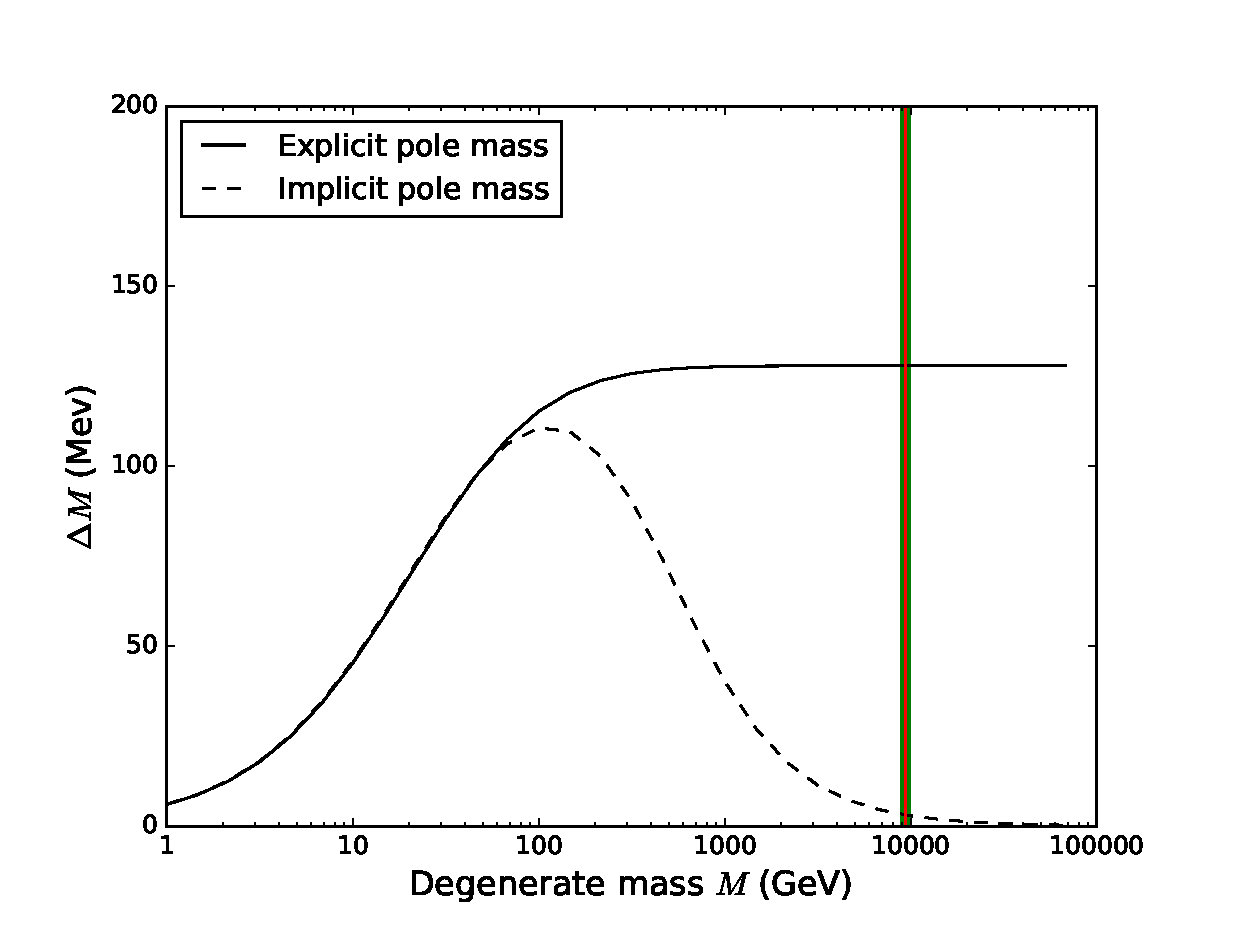
\includegraphics[width=0.5\textwidth]{mass_splittings.eps}
\caption{The mass splittings in an electroweak triplet model with a massive photon resulting from one-loop radiative corrections.  The red vertical line (and green one sigma confidence interval) indicates the physically relevant mass scale which would produce the observed relic abundance of dark matter.}\label{fig:1_loop}
\end{figure}

%
%\section{Diagnosing errors}\label{errors}
%
%In this section I give a brief outline of the possible problems that can be encountered with trying to implement new models in to \mb, along with suggested solutions.
%
%\subsection{Amplitude computation errors}
%
%The most challenging part of the \mb algorithm is the careful extraction of coefficients and basis integrals to reconstruct a given amplitude.  If the Mathematica routines encounter computational problems themselves, then this step will either succeed trivially (which may not be immediately apparent to the user) or fail.  The first step in a case where a trivial success is suspected (such as empty output files) or an error message appears is to run the same calculation with the \lstinline{-v} flag to display all Mathematica output at runtime.
%
%The case of trivial success would primarily occur when the Mathematica script is not correctly located.  In this case using the \lstinline{-v} flag will make this immediately clear.  Subsequently if the Mathematica kernel has started successfully, it will be evident from this output if the \feyncalcs, \feynarts or \tarcer packages are not properly loaded.
%
%Once it is confirmed Mathematica is running the next step is to check that all the required masses are given in the \lstinline{<model>/masses.txt} file.  If Mathematica output is being printed to the terminal, then inspection of the final amplitude displayed for any missing masses is a good starting point.  If a mass is missing, the entire computation of this amplitude must be repeated\footnote{If an extremely long calculation has been run, and only at the end was it realised a mass was missing, then it \textit{is} possible to avoid repeating it as the amplitude is saved untouched in the Mathematica data file in \lstinline{output/stage_3.mx} until being overwritten when the next amplitude is computed.  However, restarting the algorithm using this requires hacking of the code and should only be a last resort, we do not support such a feature as checking masses before hand should always be done anyway.}.
%
%
%With the trivial case aside, there are unfortunately too many possible reasons why the calculation of the amplitudes might not succeed for reasons beyond what we can control in this interface program.  However in almost all cases these problems can be resolved by looking at the Mathematica output and working through the problems for the relevant Mathematica package.
%
%
%
%
%\subsection{Compilation errors for generated code}
%
%This type of error occurs when the amplitudes have supposedly been calculated correctly, the code generated, but either the generated source code \lstinline{self_energy.cpp} or data header \lstinline{data.hpp} are corrupted.
%
%The most likely cause of this type of error is an missing coupling or constant from the input files \lstinline{<model>/couplings.txt} or a mass from \lstinline{<model>/masses.txt}.  This should be easy to identify from the compile time error for an undefined parameter which appears in the generated amplitude but for which \mb has been instructed to create a declaration for.  This is rectified by adding the required parameter to the input list and regenerating the code, the amplitudes \textit{do not} need to be recomputed.
%
%In other instances an undefined function may appear in the generated amplitudes.  These functions may some Mathematica function associated with \feyncalc or \feynartss.  Take for example the CKM mixing matrix which may be written as \cpp{CKM[i,j]} in the \feynarts model file.  \mb is not yet able to deal with \textit{functions} as couplings, but these can be added by the user manually or removed from the \feynarts model file.  In the case of the CKM matrix if quark mixing is not required this can be set to the identiy with the line \lstinline{CKM = IndexDelta} to the \feynarts model file.
%
%Generally, one may add an undefined function into \lstinline{self_energy.cpp} after code generation, or directly into \lstinline{generate_code.cpp} if it is going to be used repeatedly.  For example, the Mathematica function \cpp{Complex[a,b]} is not handled properly by the CForm output, and appears as \cpp{Complex(a,b)} in our generated output.  Therefore we add the following line to the appropriate location in \lstinline{generate_code.cpp} 
%\begin{lstterm}
%<< "TSIL_COMPLEXCPP Complex(double a,double b){TSIL_COMPLEXCPP result = a + i*b; return result ;}\n"
%\end{lstterm}
%which will print this function definition into the header of \lstinline{self_energy.cpp}.  This solves the problem of this function ever being undefined if it does appear in the generated output, and a similar approach can be followed for any function which appears in the generated output.
%
%\subsection{Choice of basis integral representation}
%
%When all possible basis integrals are constructed in \mb only unique integrals are considered.  Integrals which are equal to others, but with a different representation, for example $B(x,y) = B(y,x)$ are not explicitly added to the list.  Therefore, if some user operation which requires one of these, but by chance not the one that is in our list, problems can occur if the situation is not handled properly.  One case where this may occur is the following.
%
%It is possible, although not recommend and tedious, to construct a \tsil interface without using Mathematica at all.  The input may be directly written into \lstinline{models/output/} in the required form.  However caution must be taken to ensure all basis integrals are considered.  When the amplitude calculation algorithm is run, only a certain set of basis integrals are considered due to symmetries.  When the code is generated, only these basis integrals are searched for in the input files, using the same procedure to construct a comparison set and thus correctly read the short name formats.  For example, \lstinline{Jxyz} may be expected by the code generation routine but \lstinline{Jxzy} may not be and thus would not be identified and handled correctly.



\section{Conclusion}

I introduce a program designed to organise and simplify the use of two-loop tools for the calculation of self energies.  Although entirely an interface tool, this program makes the calculation of multiple two-loop diagrams an accessible task even on modest computing set ups.

This program provides a central structure for carrying out and storing the results of long calculations.  By producing an automatically generated interface to the \tsil libraries we enable maximum flexibility for the users choice of precomputed amplitudes to include in a calculation.

The \tsil interface provides an automated method of organising basis integrals into sets which can be evaluated using a single \tsil call, a task near impossible by hand, thus taking advantage of the structure of the \tsil libraries to speed up the calculation of the amplitude.  This is especially useful when one is switching between sets of amplitudes to compute, with the optimal combination of evaluation routines changing each time. Even as a standalone feature, this is useful to those who have already obtained a list of required basis integrals from elsewhere and intend to write their own \tsil interface.




\bibliography{../../../Papers/library}{}


\end{document}  
